%% LaTeX template for BSc Computing for Games final year project dissertations
%% by Edward Powley
%% Games Academy, Falmouth University, UK

%% Based on:
%% bare_jrnl.tex
%% V1.4b
%% 2015/08/26
%% by Michael Shell
%% see http://www.michaelshell.org/
%% for current contact information.
%%
%% This is a skeleton file demonstrating the use of IEEEtran.cls
%% (requires IEEEtran.cls version 1.8b or later) with an IEEE
%% journal paper.
%%
%% Support sites:
%% http://www.michaelshell.org/tex/ieeetran/
%% http://www.ctan.org/pkg/ieeetran
%% and
%% http://www.ieee.org/

%%*************************************************************************
%% Legal Notice:
%% This code is offered as-is without any warranty either expressed or
%% implied; without even the implied warranty of MERCHANTABILITY or
%% FITNESS FOR A PARTICULAR PURPOSE! 
%% User assumes all risk.
%% In no event shall the IEEE or any contributor to this code be liable for
%% any damages or losses, including, but not limited to, incidental,
%% consequential, or any other damages, resulting from the use or misuse
%% of any information contained here.
%%
%% All comments are the opinions of their respective authors and are not
%% necessarily endorsed by the IEEE.
%%
%% This work is distributed under the LaTeX Project Public License (LPPL)
%% ( http://www.latex-project.org/ ) version 1.3, and may be freely used,
%% distributed and modified. A copy of the LPPL, version 1.3, is included
%% in the base LaTeX documentation of all distributions of LaTeX released
%% 2003/12/01 or later.
%% Retain all contribution notices and credits.
%% ** Modified files should be clearly indicated as such, including  **
%% ** renaming them and changing author support contact information. **
%%*************************************************************************


\documentclass[journal]{IEEEtran}

\usepackage{graphicx}
% to embed the file `myreferences.bib` in your `.tex` file
% Insert additional usepackage commands here
\usepackage{color}
\usepackage{listings}
\usepackage[table]{xcolor}
\usepackage{float}
\usepackage{cite}

\graphicspath{{./Figures/}}

% Select what to do with todonotes: 
%\usepackage[disable]{todonotes} % notes not showed
\usepackage{todonotes}   % notes showed

%%% Remove the next two lines if you want the figures at their place    
%\usepackage[figuresonly,nolists,nomarkers]{endfloat}
%\renewcommand{\processdelayedfloats}{}

\setlength{\arrayrulewidth}{0.5mm}
\setlength{\tabcolsep}{10pt}
%\usepackage{courier} %caused problems for me

\def\ps@IEEEtitlepagestyle{%
	\def\@oddfoot{\mycopyrightnotice}%
	\def\@evenfoot{}%
}
\def\mycopyrightnotice{%
	{\footnotesize The copyright belongs to me!\hfill}% <--- Change here
	\gdef\mycopyrightnotice{}% just in case
}

\lstloadlanguages{% Check Dokumentation for further languages ...
	C,
	C++,
	csh,
	Java
}

\definecolor{red}{rgb}{0.6,0,0} % for strings
\definecolor{blue}{rgb}{0,0,0.6}
\definecolor{green}{rgb}{0,0.8,0}
\definecolor{cyan}{rgb}{0.0,0.6,0.6}

\lstset{
	language=csh,
	basicstyle=\footnotesize\ttfamily, 
	numbers=left, 
	numberstyle=\tiny, 
	numbersep=5pt, 
	tabsize=2, 
	extendedchars=true, 
	breaklines=true, 
	frame=b,
	stringstyle=\color{blue}\ttfamily, 
	showspaces=false, 
	showtabs=true, 
	xleftmargin=17pt,
	framexleftmargin=17pt,
	framexrightmargin=5pt,
	framexbottommargin=4pt,
	commentstyle=\color{green},
	morecomment=[l]{//}, %use comment-line-style!
	morecomment=[s]{/*}{*/}, %for multiline comments
	showstringspaces=false, 
	morekeywords={  abstract, event, new, struct,
		as, explicit, null, switch,
		base, extern, object, this,
		bool, false, operator, throw,
		break, finally, out, true,
		byte, fixed, override, try,
		case, float, params, typeof,
		catch, for, private, uint,
		char, foreach, protected, ulong,
		checked, goto, public, unchecked,
		class, if, readonly, unsafe,
		const, implicit, ref, ushort,
		continue, in, return, using,
		decimal, int, sbyte, virtual,
		default, interface, sealed, volatile,
		delegate, internal, short, void,
		do, is, sizeof, while,
		double, lock, stackalloc,
		else, long, static,
		enum, namespace, string},
	keywordstyle=\color{cyan},
	identifierstyle=\color{red},
}
\usepackage{caption}
\DeclareCaptionFont{black}{\color{black}}
\DeclareCaptionFormat{listing}

\begin{document}
%
% paper title
% Titles are generally capitalized except for words such as a, an, and, as,
% at, but, by, for, in, nor, of, on, or, the, to and up, which are usually
% not capitalized unless they are the first or last word of the title.
% Linebreaks \\ can be used within to get better formatting as desired.
% Do not put math or special symbols in the title.
\title{%
	To What Degree can an AI Built With Expert Strategies be Effective Against Competition AI?} %\\
	%\large A Planning Approach to StarCraft AI}

%
%
% author name
\author{\IEEEauthorblockN{James Hellman\\}
\IEEEauthorblockA{Falmouth Games Academy\\
UK, Falmouth\\
Email: jh182233@falmouth.ac.uk\\}
}

% The paper headers -- please do not change these, but uncomment one of them as appropriate
% Uncomment this one for COMP320
%\markboth{COMP320: Research Review and Proposal}{COMP320: Research Review and Proposal}
% Uncomment this one for COMP360
 \markboth{COMP360: Dissertation}{COMP360: Dissertation}

% make the title area
\maketitle

% As a general rule, do not put math, special symbols or citations
% in the abstract or keywords.
\begin{abstract}
Effective macro-management (the ability to create armies and expand bases), is essential to obtaining victory in Real-Time Strategy (RTS), in the research community many Artificial Intelligence's (AI's) have been created to handle this. One method is to use a design approach to create what is known as a build order, many of these build orders take from expert strategies used by real people in high ranking tournaments. Build orders can be ridged during games leaving little room for adaptation to the opponent's strategy. In this work, a collection of build orders will be used to create an AI and investigates the impact of build orders that effectively counter-strategies used by other AI's. A hypothesis is made here that the AI will only be effective in the early stages of the game and will be outmanoeuvred in late-game stages. Therefore the effectiveness of this AI will be measured its average time survived, with a high average being effective and a low average being ineffective. Whether the AI wins the matches will also be taken into account, a higher average win rate will allow the AI to face a greater challenge. Upon successful completion of this work, the AI will be submitted to one of three competitions.
\end{abstract}

\section{Introduction}
\IEEEPARstart{I}{nvestigating} the effectiveness of an AI can be done in many ways, in this work will be looking into the degree of effectiveness an AI built with expert strategies can be against a competitive AI. %First though artificial Intelligence can be defined as anything that gives the illusion of intelligence to an appropriate level \cite{AIBook}. 
In games, AI has been used in both single and multi-player environments to help create a more immersive, challenging and fun experience. One such area which AI is prominent is in the Real-Time Strategy (RTS) genre and since the call for more research to be made for AI in RTS games by Michael Buro in 2004 \cite{CallFor}, research in this area has exploded \cite{Survey}. This has given rise to the creation of many AI's in RTS games, from AI's that are built with pre-defined build orders \cite{Swen} to deep Neural Networks \cite{Deep} that can learn from game-play replays, which will be covered in more detail later on in the paper.

RTS is a great test bed in AI research for its complex systems, involving many areas of interest in planning, dealing with uncertainty, domain knowledge exploitation, task decomposition, spatial reasoning, and machine learning \cite{StarCraftBot}. Unlike turn-based strategy, RTS requires real-time decision making with imperfect information, the information is limited through the use of partial visibility of the map. Unless the AI scouts the map (Sends a unit around the map) and sees what the opponent is doing, then the AI will have no access to any strategic knowledge. This along with the non-deterministic nature of RTS, meaning it may not exhibit the same behaviour on each run, makes RTS one of the most challenging environments in which to create an AI \cite{Current}.

Since the release of StarCraft Brood War API it has been easier for Academics to research AI in StarCraft, this has also given rise to an educational value as part of AI related subjects in several Universities around the world \cite{Current}. One example of this is the University Delft (NL), which for one of its modules the students are required to create a StarCraft Bot \cite{NL}. From this three yearly competitions have been created to compete students AI's, the first of which was hosted by the University of California, Santa Cruz in 2010 as part of the AAAI Artificial Intelligence and Interactive Digital Entertainment (AIIDE) conference program \cite{AIIDE}. Another hosted at the IEEE Computational Intelligence in Games (CIG) conference \cite{CIG}, and the last one which is an ongoing stand-alone event is the Student StarCraft AI Tournament (SSCAIT) \cite{StarCraftBot}. Upon successful completion of this work, the AI will be submitted to one of these three competitions.

This paper is organised as follows, first StarCraft and what it is will be presented, followed by a review of the current methods being utilized by the research community in the development of StarCraft AI's. With a description on the research that this work will be using, this is proceeded by the method and tools that will be used to create the AI as well the metrics used to measure its effectiveness finishing with the hypothesis.
\todo[inline]{Look back to this once conclusion is done to ensure they match}

\section{Related Work}
\subsection{StarCraft}
StarCraft is an RTS game developed by Blizzard Entertainment \cite{Blizzard} and popular for testing AI \cite{Current}, the game was released in 1998 \cite{Release}. Later that year StarCraft: Brood War was released and took hold in the e-sports community and is still popular today. StarCraft 2: Wings of Liberty was released much later in 2010, with a complete visual overhaul, most of the game mechanics remained the same other than balance changes. The premise of StarCraft is to gather resources, build a base, and build an army to then use to destroy an enemies base and army, during playtime, there are also many upgrades available for these units to give them the edge over an enemy who did not spend the time acquiring them. There are many ways of doing this each player with a different order of building their armies/bases commonly referred to as their "Build Order" \cite{BuildOrder}. Build orders refer to a players macro-management, whereas in StarCraft Micro-management is a huge part of the game, as those with greater control over individual units can better outmanoeuvre their opponent, and thus defeat them. There is a difference in the way units are controlled, in StarCraft:BW you can only select up to 12 units at a time and can not group them for easy selection, so when playing you have to utilise micromanagement skills more than in StarCraft 2 where you can select an unlimited number of units and can group them for easy selection.
StarCraft is considered difficult due to its requirement of abstraction level thinking when planning. Strategy selection is perhaps the most important choice any player or AI can make in StarCraft and RTS as a whole, as this will dictate the actions and reactions which they take during playtime. Though a human player can be proficient at choosing their strategy by simply scouting the map, finding the enemy and seeing what they are building. The human player can then counter accordingly, and if they countered incorrectly the human player can simply change their strategy to accommodate. Creating an AI to do the same though can be a huge and complex task \cite{Fuzzy,OnlineEvo,GoalDriven}, one way to achieve this result without a large commitment of time is to create a library of expert strategies, and allow the AI to select the appropriate one throughout the game. This can be achieved using tools such as Advanced Behaviour Oriented Design Environment (ABODE) and Parallel-rooted Ordered Slip-stack Hierarchical (POSH) reactive plans \cite{POSH}, which will also be covered later in the paper. These tools allow for an iterative design approach for AI's in games and in this work will be focusing on the macro-management with a particular focus on build orders and the selection of strategies rather than micro-management. 

In the StarCraft research community, there are many different methods of AI creation. Some focus on micro-management like S. Liu et al \cite{EffectiveMicro} that uses a Genetic Algorithm (GA) and others that focus on macro-management looking at the build order like N. Justesen et al \cite{OnlineEvo}. Many of these research methods are cross depended and utilise more than one method, for example, D. Churchill et al \cite{Agents} created the UAlbertaBot, which was intended to automate both build order planning and unit control. There are also AI's that only use one strategy that has won several times in competitions like the ZZZKBot \cite{ZZZK,Results}, which only uses a 3pool build and built that uses a rush tactic. This rush tactic involves creating many weak inexpensive units and sending them to the enemy base within 5 minutes of starting the game. Many AI tend to struggle with countering this strategy, hence why this type of AI tends to win.

\subsection{Datasets}
A Dataset can be a collection of any data, for game AI a dataset can consist of thousands of replays with millions of game frames, and player actions\cite{Dataset}. This information can then put together to create a full game-state which allows for machine learning tasks \cite{Dataset17}. In AI research, datasets can be used in many approaches of development, one such use is to recreate game-states and evaluate them for prediction in realistic conditions \cite{SpecialTactics}.

\subsection{Micro-Management}
Micromanagement is a fundamental side of StarCraft game-play and many papers have their own approach to this aspect of RTS \cite{SOMA,EffectiveMicro,Swarm,MM,SpecialTactics,UnitsControl}. Micromanagement is the control of each unit individually, for example: if you have 12 units, each with their own ability, during battle you need to activate each ability at the correct time for each of the 12 units in order to utilise them to their full potential. This required you to select each unit during battle and activating the ability, while still maintaining control over the other 11 units. Though this is a slight exaggeration as in StarCraft some units have an auto use of their ability which allows the unit to decide when to use their ability, one such unit being the medic on the Terran faction which will heal any biological unit with less than full health. Also in StarCraft units can be selected by type i.e. you can double-click on a marine, and it will select all the marines on screen (Up to a maximum of 12). Players that perfect multitasking micromanagement skills are most likely to win the battles when playing, as they can outmanoeuvre their opponent much more easily and use abilities effectively to devastate their opponents armies. Many of these approaches tend to use either Genetic Algorithms (GA) or Evolutionary Algorithms (EA) \cite{SOMA, EffectiveMicro, Swarm}, while others observe replays and apply a Monte-Carlo method to create data for practice use \cite{MM}. But most of these methods have one thing in common, they all use a version of machine learning \cite{Survey}.

\subsection{Predictive Methods}
On a higher strategic level, the prediction of the opponent's strategy is a prominent approach used in research \cite{DataMine, Bayesian, Scouting, ReplayPred}. This type of research relies on the use of replays and machine learning to help the AI accurately predict a strategy, these do rely on the quantity and quality of replays used for the learning process\cite{DataMine,Bayesian,ReplayPred}. Another method for prediction is scouting alongside machine learning, this eliminates the need for replay observation and allows for a more real-time prediction \cite{Scouting}. Though this method does still require several games to be played before the AI can begin to have an accurate prediction.

Bayesian approaches are based on Bayes' Theorem which is another prediction method. Bayes' Theorem is a calculation of probability or also known as a probabilistic model \cite{BayesianAI}. In papers by G. Synnaeve et al \cite{UnitsControl,SpecialTactics} they create an AI that controls units individually, they do this by using uncertainty which instead of asking where a unit might be, it makes rough estimations and acts upon that. Another use for the Bayesian approach is to predict strategies, by creating a probabilistic model that after learning from replays can predict an opponent's strategy and adapt accordingly \cite{Bayesian}. A major downfall of Bayesian Approaches is that it can be computationally intense to calculate.

\subsection{Full Game Play}
Many papers try to create an AI capable of handling all aspects of an RTS \cite{Agents,Hierarchical,HumanLevel,SCAIL}. These AI's tend to take several methods that have been created in other research and combining them to form a new AI \cite{Agents}. Another use for the full gameplay AI is to try and create a "Human-Like" AI, which can mimic the play-style of an expert human player. Though the current AI's are limited in this as players reported that the AI's used unusual unit movements or building placement \cite{EvalHuman}.

\subsection{Neural Networks}
Neural Networking are computational models loosely based on the functioning of biological brains \cite{Deep}. Given an input it computes an output by using a large number of neural units, in StarCraft it can be used to predict strategies or in the case of StarCraft 2 with its new architecture it can be used for full game-play. Using a neural network would be impractical for the purpose of this work as it would take many months to train, and even then would not have a great chance of doing well against other AI's.

\subsection{Planning}
Planning in StarCraft usually deals with the build order that the AI will use usually only dealing with macro-management. There are several different ways to use a build order, some will use a static build order that will not change throughout the game \cite{Swen}, and the more popular route is to allow the AI to jump between build orders during play-time, another term is Reactive Planning \cite{Fuzzy,OnlineEvo,GoalDriven}. there has been some work on creating the build orders on the fly by finding out that most optimal method of gathering resource and building units \cite{BuildOrder}. Planning is perhaps the most optimal approach to creating an AI as there are little real-time calculations to make. Through the use of POSH tools \cite{POSH}, you can iteratively design AI prototypes and deploy quickly \cite{Swen}. 

From looking at the research in the field there are many methods that can be used to create an AI. The use of replays to train an AI to counter strategies can be effective \cite{Bayesian}, they lack the greater control of the game, the ability to macro-management as there are too many variables to consider. This lack of large-scale control is usually due to the heavy computational requirements of controlling each individual component of the game.  Due to this slow process, it is quite impractical to use when there is already a library of knowledge that can be to exploited \cite{Liquid}. Though there are AI's out there with planned strategies already programmed into them \cite{ZZZK,Fuzzy}, their limitation is that they only use a small number of strategies, though these work it can leave a lot of room for the opponent to manoeuvre. A logical step here is to program a larger pool of expert knowledge into the AI, it will then select one and follow it through, with the ability to jump between strategies at key points in-case a counter is detected. 

\subsection{StarCraft AI's}
In the StarCraft AI community there are many AI's that have been created to compete against each other, and in this work, a competition AI is defined as an AI that has been entered to the AI for Interactive Digital Entertainment conference (AAIDE) StarCraft AI Competition. A yearly competition hosted by David Churchill and sponsored by AIIDE. Examples of the top AI's from the competition include:
\begin{itemize}
\item ZZZKBot Winner of the 2017 AIIDE StarCraft AI Competition \cite{ZZZK} 
\item Iron Winner of the 2016 AIIDE StarCraft AI Competition \cite{Iron}
\item UAlbertaBot Winner of the 2013/2011 AIIDE StarCraft AI Competition \cite{UAlberta}
\item Skynet Winner of the 2012 AIIDE StarCraft AI Competition \cite{Skynet}
\end{itemize}

Each of these bots employ different strategies, these strategies a
\todo[inline]{Discuss the other bots and their strategies}

\subsection{Research Questions and Hypothesis}

\subsubsection{Hypothesis}
\begin{itemize}
	\item \textbf{Hypothesis 1} The AI will survive no more than 13 minutes in a match with the inbuilt AI.
	\item \textbf{Hypothesis 2} The AI will survive no more than 13 minutes in a match with the competition AI.
	\item \textbf{Hypothesis 3} The AI will defeat the inbuilt AI
	\item \textbf{Hypothesis 4} The AI will defeat the competition AI.
	\item \textbf{Hypothesis 5} The AI will counter the Rush tactic.
\end{itemize}

\subsubsection{Research Questions}
During the initial research into this area for this paper other research questions were reviewed:
\begin{itemize}
	\item Combining Behaviour Oriented Design and Expert Human Knowledge to create a competitive AI.
	
	\item Creating an adaptive AI using predefined expert strategies. 
	
	\item Is an adaptive AI built with predefined expert strategies a viable competitor against non adaptive AI’s?
	
	\item How effective can an adaptive AI built with predefined expert strategies be against other AI’s?	
\end{itemize}
These questions were rejected as creating an adaptive AI was not the focus of this research.
\newline

\section{Method}

\todo[inline]{Empirisism} 
\todo[inline]{Include some philosophy on this paper (positivist research)}

This research will employ a positivist approach in its philosophy, meaning that during the design, implementation and execution of the experiment.....

In this work Protoss will be chosen, this choice was made as Zerg have been done many times and usually rely on rushes to win, whereas Terran are too complex for the planned AI. Protoss proved a happy middle ground to build upon where rushes are difficult to achieve but they are not too complex that it is too difficult to execute a sound strategy. So the second logical step is to implement an anti-rush strategy as an opening strategy. From there more aggressive strategies will be implemented and executed at the appropriate times. The challenge here is that it is difficult for Protoss to counter a Zerg rush but if successful it will leave the Zerg open for attack. To support this decision the ratio that the races won were looked into and can be seen in fig 4, here the Protoss clearly loose more often than the other two races.

\subsection{Tools}
The tools that will be used in this experiment are; The Brood War Application Programming Interface (BWAPI), POSH tools, specifically POSH Sharp which is an interface that uses c\# instead of C++, and the ABODE editing software which uses POSH plans to create Behaviour Oriented Designs for AI's. Other tools include Visual Studio 2010, Chaoslauncher, StarCraft Tournament Manager, and VirtualBox, all of which will be explained next. 


\begin{figure}[H]
	\centering
	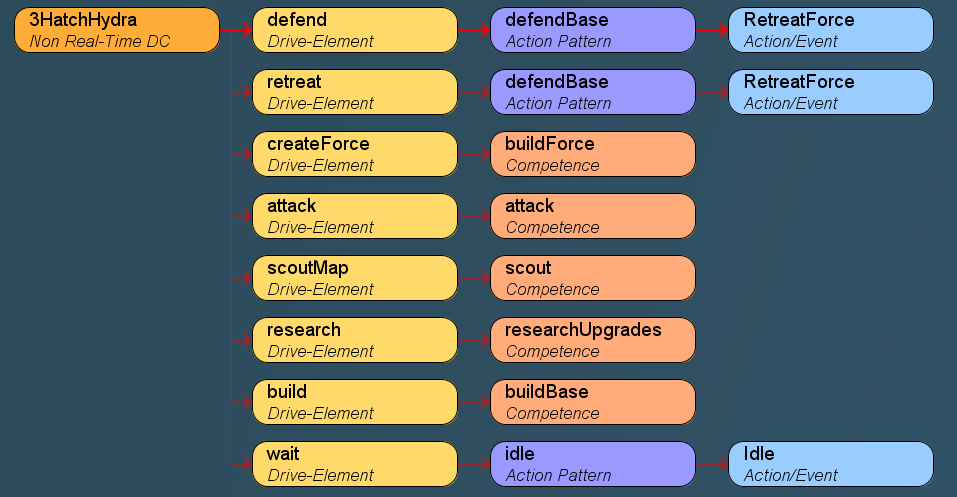
\includegraphics[width=0.5\textwidth]{POSH}
	\caption{POSH plan for the Three Hatch Hydra build plan inside the ABODE editor.}
	\label{Fig1}
\end{figure}

\begin{itemize}
	\item \textbf{Brood War Application Programming Interface} \cite{BWAPI} is an open source software that creates an interface to allow a custom AI to communicate with the game. BWAPI only give limited information to the AI, which inhibits the bots to have the ability to know what its opponent is doing, this means that the fog of war(the unexplored parts of the map) are is kept\cite{POSH}, this mean that the AI is just a limited in its knowledge as a player would be. The information that is provided is the size of the map and base locations, this allows the AI to have the ability to scout effectively. This limited information prevents custom AI's from cheating and ensures a fair game, though for the developers of the AI this could be considered an advantage for the development stage of the AI as there is no need to be concerned with accidentally allowing their AI to access illegal information. This does however provide a challenge in design as the AI is dealing with imperfect information, it must be designed in such a way that it almost replicated human responses, i.e. scouting, and checking areas already scouted for enemy presence.
	\item[]
	\item \textbf{POSH} plans can be created in the ABODE Environment as seen in Figure 1, these are visual planning tools that allow for a hierarchy of actions with associated triggers. Each plan can be split into three parts, Drive-Collections, Competencies and Action patterns, these three determine when an action is to be triggered. POSH plans use a behaviour library created in the native language of the problem space, see Fig 1. This tool can be a powerful asset to designing and creating an AI as once the behaviours and senses are implemented new AI can be created quickly and with little error.
	\todo[inline]{Mention the many (((((()))))) language here}
	\item[]
	\item \textbf{Microsoft Visual Studios 2010(VS2010)} is an integrated development environment(SDK) from Microsoft \cite{Visual}. It is used to create computer programs, as well as websites, apps, and online services. In this experiment VS2010 is being used to create the behaviours for the AI, as well as any other functionality the AI requires, this includes the framework for the POSH wrapper.
	\item[]
	\item \textbf{Chaoslauncher} is an open source third-party launcher for StarCraft that allows the user to inject any universal plugins \cite{Chaos}. For this experiment the launcher will be used as a debugging tool for the first stages of the AI. The launcher also allows StarCraft to be run in windowed mode alongside a BWAPI injector that allows the AI to communicate with BWAPI.	
	\item[]
	\item \textbf{StarCraft AI Tournament Manager(STM)} is a tool that was developed by David Churchill to manage and run StarCraft AI tournaments, it is an open source project available for anyone to use. It runs the tournament by creating a server and allowing instances of its counterpart (the Client) to connect to it, each client runs a single instance of StarCraft and the server will put two clients into a game and record the results. This set-up allows for as many instances of StarCraft to be run on the server as the user wants, unfortunately the current set-up of the STM doesn't allow for more than one instance of StarCraft to be run on a single PC at a time. To solve this a virtual machine will be utilized \cite{Tournament}. For the purposes of this experiment the STM will be used to test the AI against the competition AI's, once the tournament is over the STM will compile  a results table similar to fig 2, in a HTML format which can be opened in any browser.
	\item[]
	\item \textbf{Oracle VirtualBox} is a general-purpose full virtualizer for x86 hardware, targeted at server, desktop and embedded use \cite{Virtual}. This allows the user to run multiple instances of an operating system on the same hardware, for this experiment it will be used to run multiple instances of StarCraft on the same PC. 
\end{itemize}

\begin{figure}[H]
	\centering
	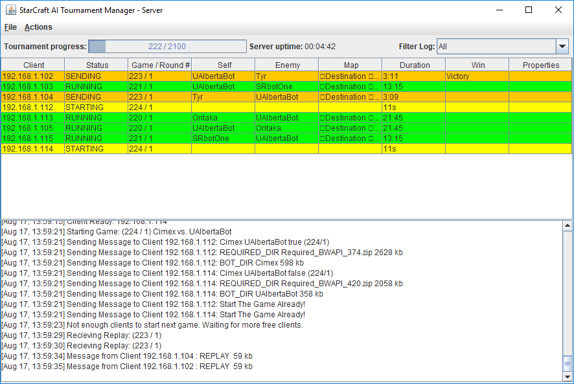
\includegraphics[width=0.5\textwidth]{TMPic}
	\caption{StarCraft Tournament Manager Server Running.}
	\label{Fig2}
\end{figure}

\subsection{Design and Research Artefact}
Designing this experiment was a simple task once the research question was settled on, as the only designing required was to obtain several expert strategies. These strategies were obtained from an online source Liquipidiea, this is an online wiki available to the esports community to bring together all the information they can to help each other in their respective sports. This wiki is a valuable source of knowledge when trying to obtain the necessary StarCraft strategies as the ones on this site are used by the experts that play the game. 

The challenge was the implementation of these build orders, as the POSH plans have to be precise, meaning the priorities of its actions had to be correct, plus the timing of each action needed to be correct. 

This work will be focusing on the implementation of an AI with pre-built build orders and their counters taken from Liquipedia \cite{Liquid}, a website dedicated to StarCraft, on the there they have a collection of strategies that are free to use in any capacity. Building upon these build orders, the experiment will also include a method for swapping between the orders at any point, to know when to do this, the AI will scout the map in search of the opponent and compare their current building to its stored build orders and find an appropriate counter. The issue with this method is that in late game the AI will struggle to decide which build order to continue. 

\begin{figure}[H]
	\begin{lstlisting}
[ExecutableAction("SelectProbeScout")]
public bool SelectProbeScout()
{
    if (probeScout != null && probeScout.getHitPoints() > 0)
        return true;

    Unit scout = null;
    IEnumerable<Unit> units = Interface().GetProbes().Where(probe =>
    probe.getHitPoints() > 0 && !Interface().IsBuilder(probe));

    foreach (Unit unit in units)
    {
        if (!unit.isCarryingGas())
        {
            scout = unit;
            break;
        }
    }
    if (scout == null && units.Count() > 0)
    {
        scout = units.Last();
    }
    probeScout = scout;
    return (probeScout is Unit && probeScout.getHitPoints() > 0) ? true : false;
}
	\end{lstlisting}
	\caption{c\# executable action for selecting a probe scout, the plan will execute this code when triggered.}
	\label{Fig3}
\end{figure}
\todo[inline]{Talk about the lifecycle of the artefact agile test driven development TDD no use of daily scrums.}

This artefact used Agile and Test Driven Development(TDD) or in terms of this artefact it will refer to Test-Driven Design for its lifecycle. In K.Beck's Book: Test-Driven Development By Example (cite), TDD as a development concept follows two rules:

\begin{itemize}
	\item Don't write a line of new code unless you firs have a failing automates test.
	\item Eliminate Duplication
\end{itemize}

These two rules 
\todo[inline]{Expand on this}
Testing in this instance was only concerned with whether a function within the code did as was designed, there is only a pass/fail did it do the thing it was designed for or not, when testing these only one test is usually required to ge the answer then a slight modification was made each time if it resulted in a fail. The tests had only minor automation as the artefact had to be manually run and the game manually set-up.
\newline

\subsubsection{Sprint 1 : Software Installation}
The first sprint was to set up the environment. This involved downloading and installing several versions of Visual Studio, and downloading the correct version of BWAPI, Chaoslauncher, and the addition of PoshSharp. An intimidate issue that came up after attempting to compile BWAPI, there were missing .ddl's in the Windows directory, to rectify this the relevant dll's were manually copied into the relevant locations. Once the coding environment was set up, the next step before any code was written was to set up the testing environment. This was done using the Chaoslauncher, BWAPI had to compile correctly to begin with otherwise the AI would not inject into the game correctly. Once StarCraft launched with no issues, a basic POSH plan with no functionality, that came with POSHSharp was compiled and executed, this all had to be done in admin mode as it would not work correctly. By the end of this sprint the correct software was installed, the testing environment was working, and a basic plan ran in the game. The artefact at this point was ready to be designed and have code written in the behaviours.
\newline

\subsubsection{Sprint 2 : Prototype}
For the prototype stage of the artefact a race had to be chosen, in StarCraft, there are three, Zerg, Protoss and Terran, each with their own unique play style. Zerg is a rushing faction, with their units being relatively weak and cheap, Zerg usually focus on overwhelming their enemy with numbers. Protoss are strong but expensive, relying on smaller numbers and taking longer to produce anything, this means they can be weak at rushing and defending from a rush. Terran is a balance of the two, being able to produce strong and expensive units as well as cheap, weak ones, they can effectively rush and defend from a rush.

A rush is a tactic employed in RTS games which involves building up a small force as quickly as possible to harass the enemy base and units. A rush is only considered a rush if it is done within the first five minutes of the game \cite{Liqui}.

The artefact needed to have an executable plan for the desired race, in this case Protoss, the reasoning for this is explained in the Method section, under Preliminary Results. No behaviours were changed, this was simply an exercise to ensure the testing environment ran with the correct race, so only basic functionality was present. In this case the Probes would gather resources and build a Pylon. This would be the final step in setting up the tests, as now the Protoss ran with no issues in game and testing would be seamless.
\newline

\subsubsection{Sprint 3 : Alpha}
Creating an alpha involved changing the behaviours to suit the race and the behaviours that came with the software were written for Zerg only. Which meant that there had to be a lot of redesigns and code re-factoring needed. And example of this would be the positioning of buildings, as for Zerg they can only build on something called "Creep" this is present at the start of the game at a set radius around the starting base, and can be extended through the use of special structures. For Protoss however they can only build within range of a structure called a "Pylon", these Pylons can be built anywhere but any other structure bar the starting structure has to be built within range. The behaviour for the placement of structures for Zerg worked fine for them however for the Protoss the function had to be refined for more precision when building. 

Another example is when building structures the Zerg loose a builder, as the builder "Morphs" into the structure so each time something is built the AI would just select a new builder and remove the previous one from any list it was related to. Protoss on the other hand can have many structures constructing at one time, this means that the build must remain the same unit. Plus the Training of units, as Zerg only trained from one structure where as Protoss would train from several.

This was done over several weeks, every behaviour, action and sense that was modified/written was tested for functionality each and every time there was a change. This allowed the artefact to take small steps with each change and test always progressing. Once a piece of code was complete there was rarely a need to return to it, and if there was then it was a simple matter to make a change and test if it worked. By the end of the sprint the AI was building in the correct places and produced units from another structure.
\newline
\todo[inline]{Reasonable plan with most basic behaviours working}

\subsubsection{Sprint 4 : Beta}
During this sprint the objective was to ensure the AI could build in other locations as well as build an army to attack the enemy. The first goal was to create a method for the AI to find the choke point and set it as a base location for building, this also opened up an issue with ensuring the AI can swap building locations. Within BWAPI the AI has knowledge of all the choke points and base locations, though they are not allowed to access them unless it has been revealed on the map. then once it has the AI can save that location, and once it needs to build there it will use the positioning code from that location instead of from the start base. 

Once the functionality for building at the choke was implemented and tested, a plan with greater detail was created. Meaning that the AI would now take advantage of building at both the starting area as well as the natural expansion and choke point. Along with this the AI had to build an army and attack the enemy, using the new method for finding new build locations, it was a simple modification to the scouting function to allow the AI to find the enemy base and mark its location, which allowed the AI to know where to go with its forces.

During this sprint it became clear that the strategies provided from Liquipidia were not going to work, as they relied on the player (AI) scouting and building immediately as the game started. Unfortunately as the system can not compute its actions instantaneously the AI can not execute the strategies in time before the enemy AI had wither rushed or build a larger force. This proves my null hypothesis in these conditions, being the framework is too slow and needs altering, and as this was not the focus of this research would have been an improper use of resources.

To counteract this The AI has been modified to include a tactic that is not present in any of the strategies, which is to build several Protoss Photon Cannons at the natural expansion. This means that the base immediately next the the AI's starting position will be built up with defensive structures to stop any early game threat, allowing the AI to continue with the original strategy proposed.
\newline
\todo[inline]{Mostly complete plan most behaviours working}

\subsubsection{Sprint 5 : Polish}
At the end of this sprint the AI was expected to have all behaviours fully implemented and tested and a completed plan written and tested. This was an opportunity to look back and re-factor any code that needed tuning or any duplicate code that got into the system. Though the point of TDD is to avoid duplicate code, its priority is to get code that works, in the case of this software duplicate code did end up in the system. Unfortunately due to the nature of the "Action", "Sense" system there is bound to be duplicate code, though it can be minimized with internal functions.
\begin{table*}[]
	\centering
	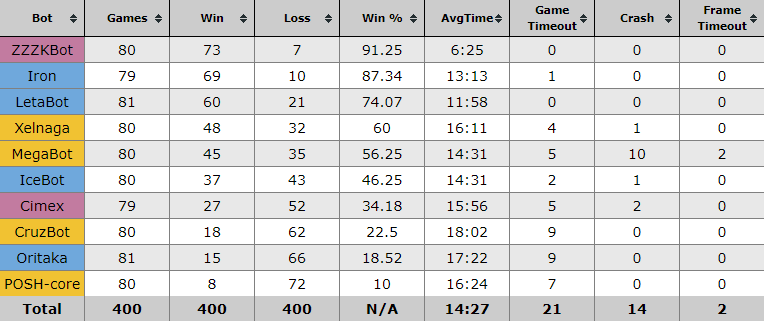
\includegraphics[width=\textwidth]{STMResultsWithBot}
	\caption{The HTML results table produced by the StarCraft Tournament Manager \cite{Tournament}. Blue represents Terran, Purple represents Zerg, and Yellow represents Protoss}
	\label{Table1}
\end{table*}
Tuning the plan took most of the time in this sprint as with each change the plan had to be tested within the game, to ensure that th change was meaningful and effective. This usually involved changing the build order and priority order of actions.
\newline
\todo[inline]{Complete plan and complete behaviours with tuning}
\subsubsection{Sprint 6 : Implementation of New Strategies}
The final sprint was to implement several plans that could work alongside the base plan, these would all be taken from the Liquipidiea site. Unfortunately the current set-up only allows for one plan to be used at a time, though each plan can contain several strategies that are triggered when the AI plays.
\newline

\subsection{Preliminary Results}
To prepare for final testing a preliminary test was carried out using the tournament manager, this was done to ensure the software was set-up and working for the final testing for the AI developed for this research. For the preliminary test 9 AI's were chosen from the AIIDE 2016 competition, three from the top, three from the middle and three form the bottom. These bots would then play one on one games on 10 maps, totalling to 360 games, the results of each match were recorded automatically by the tournament manager and compiled into table 1, from this table fig 4-8 were created. These results allowed the further development of this researches metrics, this is explained in the following section.

because the times are only for the games that have that bot in it

\begin{figure}[H]
	\centering
	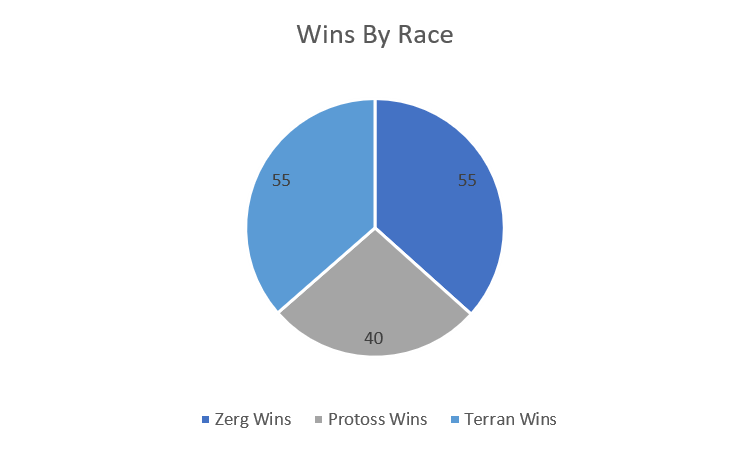
\includegraphics[width=0.5\textwidth]{RacePie}
	\caption{A pie chart representing the average win rate \% for the three races, based on the results obtained from table 1.}
	\label{Fig4}
\end{figure}
\begin{figure}[H]
	\centering
	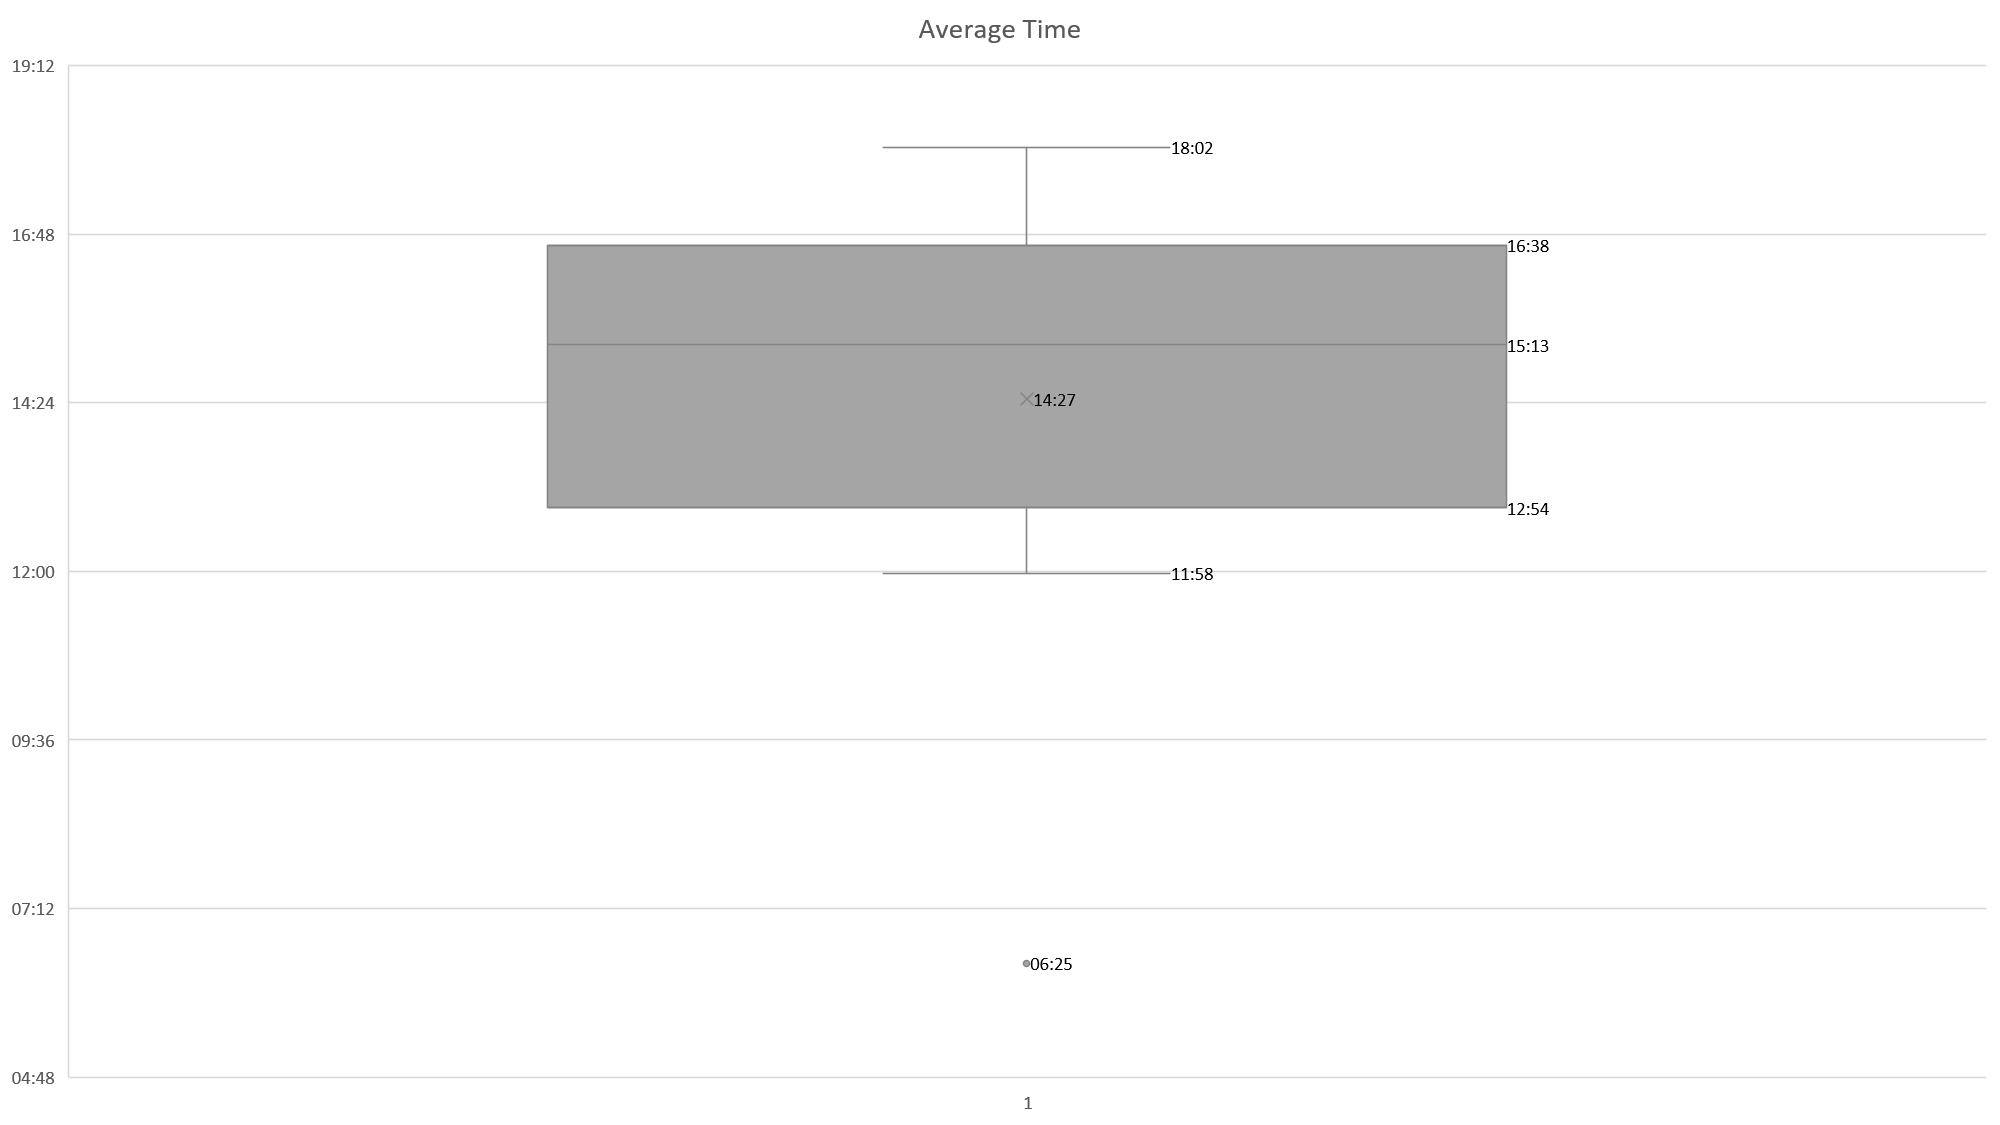
\includegraphics[width=0.5\textwidth]{AvgTimeBarBot}
	\caption{Box and whisker showing the average game length, with the mean, median and outlier based on the results obtained from table 1.}
	\label{Fig5}
\end{figure}
\begin{figure}[H]
	\centering
	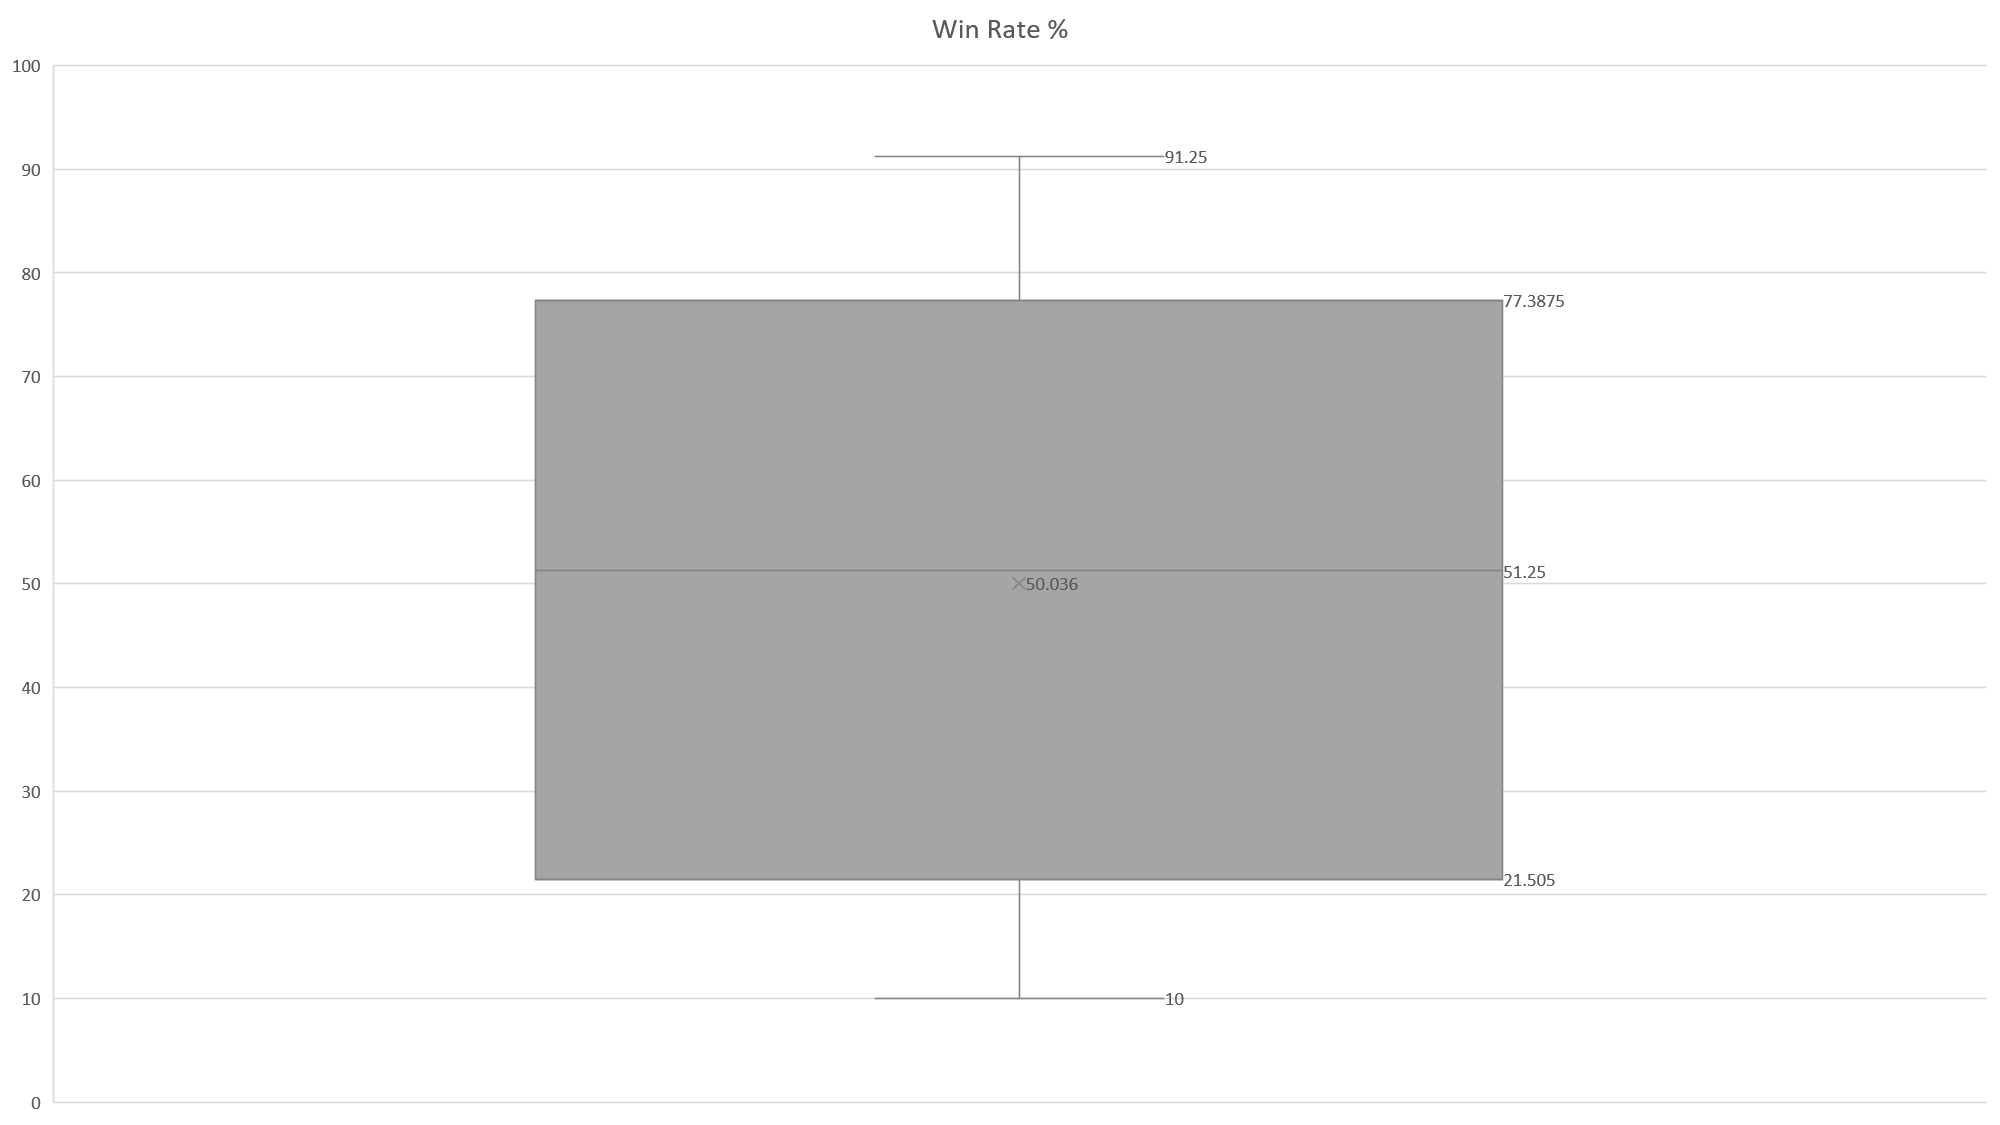
\includegraphics[width=0.5\textwidth]{WinBarBot}
	\caption{Box and whisker showing Win Rate, with the mean and median based on the results obtained from table 1.}
	\label{Fig6}
\end{figure}
\begin{figure}[H]
	\centering
	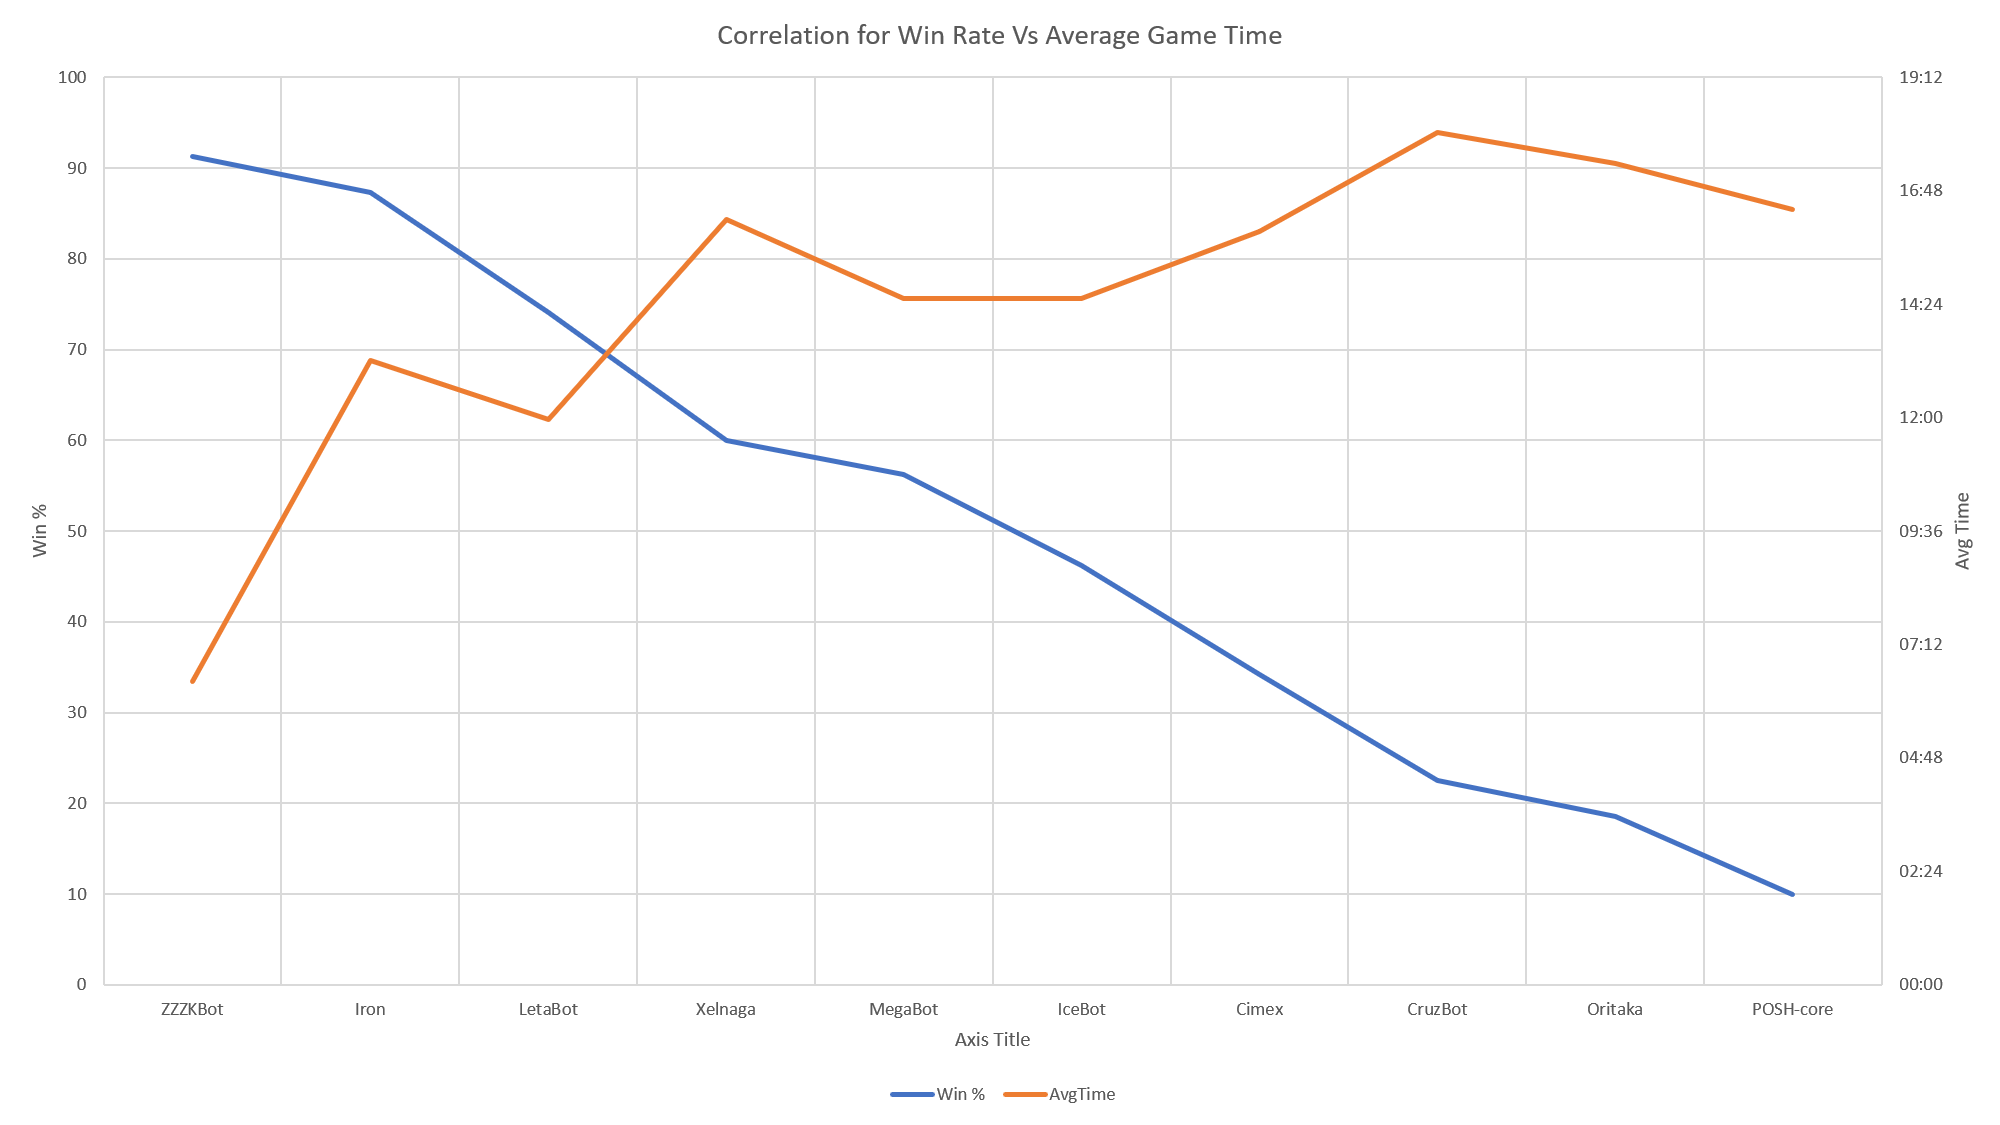
\includegraphics[width=0.5\textwidth]{WinTimeLineWithBot}
	\caption{A line graph showing both the win rate and game length for all the bots, starting with the highest win rate on the left, based on the results obtained from table 1.}
	\label{Fig7}
\end{figure}
\begin{figure}[H]
	\centering
	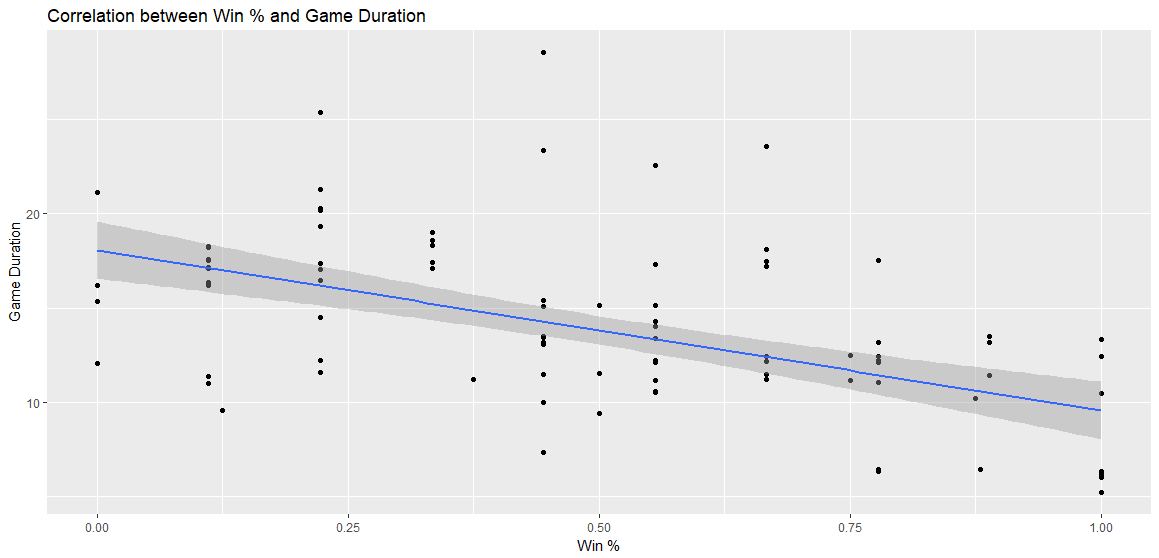
\includegraphics[width=0.5\textwidth]{ScatterWinvsDurLine}
	\caption{A scatter plot showing a negative correlation between the win rate and game length, based on the results obtained from the preliminary experiment. Each dot represents an average win rate and average game length for each bot during each round.}
	\label{Fig8}
\end{figure}
\subsection{Metrics}

Initially the StarCraft AI was to be measured on its success in these two metrics:
\begin{itemize}
	\item \textbf{Time Survived} (Average of 13 minutes or above)
	\item \textbf{Endgame Condition} (Whether the AI wins the game or looses)
\end{itemize}
These metrics were obtained from the results from the AIIDE which found that the average time of each game was 13-minutes, and the quickest average being 8-minutes and the longest being 19-minutes. The win ratio of the AI's vary substantially from 17.21\% to a high 83.11\% as can be seen in Table 1 \cite{Results}. 

After presenting these findings, it was discussed that the metrics required a greater level of merit, to achieve this, the metrics were modified using the preliminary results and further inspection of the AI's within the literature. As can be seen in fig 6, the mean win rate for the AI was 50\% and the mean game length from fig 5 was 14.20, and within the literature the only concern for some papers were win rate, these range from 54-91\% \cite{ELGoal,Swen,OnlineEvo,GoalDriven}. The literature AI's were faced against both competition AI's and in-built AI's, which means their win rates could be inflated.

No papers that were reviewed for this research focused on average game length, though for the purposes of this research it will be. As can be seen in fig 8 and 9 there seems to be a negative correlation between win rate and game length, which supports the metric.
\newline

For the final metrics that the AI will be measured on will be as follows:
\begin{itemize}
	\item \textbf{Average Game Length} (Average of 14 minutes or below)
	\item \textbf{Average Win Rate} (Win Rate above 50\%)
\end{itemize}

Through these revised metrics, the effectiveness of the AI will be determined, if the AI obtains an average game length of 14 minute or less, and or has a win rate of 50\% or higher it will support the statement that it is effective. Though if the AI fails at achieving these goals it will support the NULL hypothesis.

\subsection{Testing}

To begin with, the AI will be pitted against the inbuilt AI as a test-bed, playing 10 matches against the three races. 10 is chosen as if the AI should win each game and or survive well into the upper range then there will be little reason to continue testing against the inbuilt AI as it will most likely continue this way. After the initial testing, the AI will then be put against an open source competition grade AI, and 100 games for each AI will be simulated. This number has been chosen as it will give a total of 400 games and will provide strong evidence to support the hypothesis presented here.

During testing there will be a total of 10 AI's including the AI that was developed for this research. To choose these AI's three were selected from the top of the board, three from the middle and three from the bottom. They will be selected from the AIIDE 2016 competition, to keep the experiment af fair as possible each AI in each tier will consist of each of the races, where that is not possible, a substitute will be made \cite{2016}. AIIDE 2016 was chosen as all the bot's required for testing were available for download.

The 10 AI's will be playing on a total of 
\todo[inline]{Mention that the testing will be within a competition environment.}

\todo[inline]{Talk about how and what you are testing}

\subsection{Disadvantage of Software}
Though once this system is complete with all the behaviours needed are present, makes it quick and easy to create new AI plans, it has one major disadvantage. The AI can only execute one action at a time, for example, when the executes the "ProbeScoutToEnemyBase" action it must wait for the entire action to be executed before moving on to the next. This has a negative effect on the design of the AI as it must be created in such a way that it can be effective while being limited to only one action at a time.

Another issue presented by this software is that it is CPU intensive and slows down the game simulations considerably, this will make testing time increase and unfortunate there is not much that can be done about it, as the c\# is being translated into c++ for the BWAPI to translate into StarCraft commands.


\section{Results}
\todo[inline]{Describe the results do not discuss}

\section{Discussion}
\todo[inline]{Talk about the results and the implications}


\section{Professional Considerations}


\section{Future Work}
Though the null hypothesis was confirmed, this work provided an interesting find, that there is a possible correlation between the win rate and win time. A proposed question for future work would be if there is a correlation between them. This would be an interesting find as it could be used to alter the design of AI's to facilitate fast strategies, and through the Zerg implemented a rush tactic which is inherently fast, it would be interesting to see how and AI using Terran or Protoss would cope with similar strategies.
Altering the artefact to have executable time set as a priority during development would be an advantage for this as the current software can not keep up with the other AI's in its current state.

An alternative option to solve this issue is to create another plan to run in parallel to the original. This will allow the AI to execute multiple behaviours at the same time, rather than executing one and having to wait for it to finish before moving on to the next. This would, for example, allow the AI to build up their base, scout and manage their army at the same time. Unfortunately it would involve precision planning as each plan would have to ensure they do not execute the same action at any point. This was not the primary focus of the artefact, as the framework would have to be modified to allow the use of parallel plans.

Using parallel plans would provide an interesting premiss for designing an AI. The AI could have multiple plans, each focusing on a separate component of the game, these could be combat, base building, resource management or defence. Creating an AI with this capability would provide a challenge in its design as the plans would have to communicate with each other to allow the correct execution times, and it would have to ensure there are no conflicts of interest when managing units. This could be solved with a order of priority or a threat calculation, so the defence can take over from the combat plan if the AI is loosing its base.

A further step that could be taken is to allow the AI to construct its own plans with neural networking. It would allow the AI to learn from pre-built strategies and alter them accordingly as it played a number of matches.

\section{Conclusion}
\section{Acknowledgements}

% references section

\bibliographystyle{IEEEtran}
\bibliography{references}

\section{Reflective Addendum}
\todo[inline]{FOR EXAMPLE: During this dissertation many challenges had to be overcome, in subsection those challenges will be explored.}

% Appendices
\appendix
\begin{table*}
	\centering
	{\rowcolors{3}{green!80!yellow!50}{green!70!yellow!40}}
	\begin{tabular} { |p{3cm}||p{1.5cm}|p{1.5cm}|p{1.5cm}|p{1.5cm}|p{1.5cm}|  } 
		\hline
		\multicolumn{6}{|c|}{2017 AIIDE StarCraft AI Competition} \\
		\hline
		Bot & Games & Win & Loss & Win\% & AvgTime\\
		\hline
		ZZZKBot	&	2966	&	2465	&	501	&	83.11	&	8:00	\\
		PurpleWave	&	2963	&	2440	&	523	&	82.35	&	13:27	\\
		Iron	&	2965	&	2417	&	548	&	81.52	&	14:19	\\
		cpac	&	2963	&	2104	&	859	&	71.01	&	9:45	\\
		Microwave	&	2962	&	2099	&	863	&	70.86	&	11:34	\\
		CherryPi	&	2966	&	2049	&	917	&	69.08	&	9:50	\\
		McRave	&	2964	&	1988	&	976	&	67.07	&	14:35	\\
		Arrakhammer	&	2963	&	1954	&	1009	&	65.95	&	11:37	\\
		Tyr	&	2966	&	1955	&	1011	&	65.91	&	13:09	\\
		Steamhammer	&	2964	&	1901	&	1063	&	64.14	&	10:32	\\
		AILien	&	2966	&	1729	&	1237	&	58.29	&	13:04	\\
		LetaBot	&	2955	&	1682	&	1273	&	56.92	&	16:48	\\
		Ximp	&	2962	&	1605	&	1357	&	54.19	&	18:46	\\
		UAlbertaBot	&	2968	&	1585	&	1383	&	53.4	&	10:54	\\
		Aiur	&	2965	&	1496	&	1469	&	50.46	&	13:51	\\
		IceBot	&	2955	&	1348	&	1607	&	45.62	&	17:16	\\
		Skynet	&	2958	&	1295	&	1663	&	43.78	&	11:40	\\
		KillAll	&	2965	&	1276	&	1689	&	43.04	&	10:56	\\
		MegaBot	&	2802	&	1200	&	1602	&	42.83	&	12:21	\\
		Xelnaga	&	2962	&	1099	&	1863	&	37.1	&	15:19	\\
		Overkill	&	2958	&	967	&	1991	&	32.69	&	18:00	\\
		Juno	&	2962	&	876	&	2086	&	29.57	&	14:07	\\
		GarmBot	&	2961	&	802	&	2159	&	27.09	&	15:21	\\
		Myscbot	&	2964	&	769	&	2195	&	25.94	&	13:41	\\
		HannesBredberg	&	2964	&	630	&	2334	&	21.26	&	14:09	\\
		Sling	&	2963	&	625	&	2338	&	21.09	&	16:21	\\
		ForceBot	&	2960	&	532	&	2428	&	17.97	&	15:10	\\
		Ziabot	&	2964	&	510	&	2454	&	17.21	&	10:08	\\
		Total	&	41398	&	41398	&	41398	&	49.98	&	13:23	\\
		\hline
	\end{tabular}
	\caption{Results of the 2017 AIIDE StarCraft AI Competition Sourced from the official website \cite{Results}}
	\label{table2}
\end{table*}


\newpage
\listoftodos[Notes]

% that's all folks
\end{document}
